\documentclass[12pt]{article}
\usepackage{graphicx}
\graphicspath{{Figures/}}
\addtolength{\textwidth}{1in}
\addtolength{\textheight}{1in}
\addtolength{\evensidemargin}{0.5in}
\addtolength{\oddsidemargin}{-0.5in}
\addtolength{\topmargin}{-0.5in}
\title{Galaxy Formation}
\author{Sina Babaei Zadeh\\SURP}
\date{\today}
\begin{document}
\maketitle

\begin{abstract}
SURP project introduction. In this kick off mini project, we will gain a basic understanding of galaxies and become familiar with the tools needed to understand galaxies, especially their formation using the data collected by the Eagle Project.
\end{abstract}
\tableofcontents
\clearpage 

\section{Introduction}
This is a short mini project to start my the SURP program. We will be analysing data from the Eagle Project, in particular focusing on the main formation. In part, we will explore red-shifts, queries, and other interesting results and data.
\begin{figure}
  \centerline{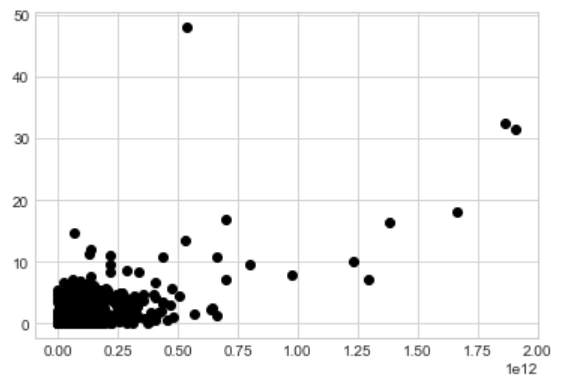
\includegraphics{Galaxy.jpg}}
  \caption{Galaxy formation without log (bad scale). A better version shall be used in the following sections. Our analysis will focus on these types of data taken from the Eagle Project.}
  \label{fig:picture}
\end{figure}




\section{Results}

We will present the result of our galaxy analysis using data collected by the Eagle Project. 




\subsection{Our First Query}

The query is an array containing the stellar mass of a galaxy and its respective star formation rate. Various galaxies with red-shift zero are tracked over a time span and their information is collected by the query. There are various conditions placed on the query such as including SnapNum=28 galaxies which corresponds to the zero red shifted ones, and other conditions such as stellar mass being considered be greater than zero. Depending on our conditions, we receive different data which impacts our plot. Alternatively, we could have used the Red-Shift column to achieve the same results.

\subsection{Going in deeper}

\begin{figure}
  \centerline{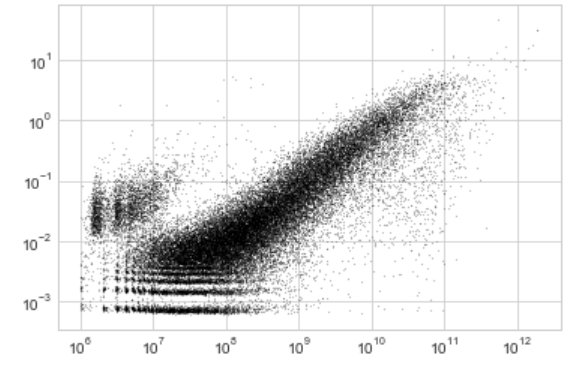
\includegraphics{d.png}}
  \caption{Galaxy formation with log scale (zero red-shift)}
  \label{fig:picture}
\end{figure}

The figure above is the main sequence galaxy formation for zero red-shifted galaxies. As we can see, most galaxies occupy the middle which means that they have average stellar mass and average star formation rates. This implies that they are not too old, but not too young either. Since the young galaxies would have little mass (x-axis), but a high rate of new star formation (y-axis). This makes sense because new galaxies are still gathering up mass, and stars are forming rapidly from the clumps of available gas. 

Conversely, the older galaxies would have a lot of mass, but little activity (new star formation). Since most of the mass would already be in the Black Holes and already created stellar objects leading to a lack of gas clumps that could give rise to new stars. Therefore, these galaxies would have high mass (x-axis), but low star formation rate (y-axis). 

Although this model is very useful, it is not identical to what we observe nature. This is because a galaxy could show up multiple times with different time scales and data. Hence, the data looks very continuous instead of having sharp distinctions between the middle part (Average galaxies) and the bottom and top clusters for old and new galaxies respectively. Furthermore, the figure doesn't show galaxy sets in the process of developing such as becoming middle age or old and looks more like a blob. Another problem with this figure is that it only accounts for zero red shift galaxies, so it doesn't convey the whole picture. In the next section we will see no-zero red shifted galaxies.
\begin{figure}[h]
  \caption{Galaxy formation with log scale (0.5 red-shift)}
  \centering
  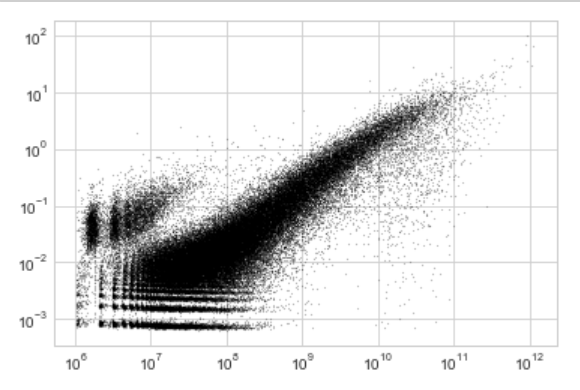
\includegraphics[width=0.5\textwidth]{g.png}
\end{figure}

\begin{figure}[h]
  \caption{Galaxy formation with log scale (0.5 OR LESS red-shift)}
  \centering
  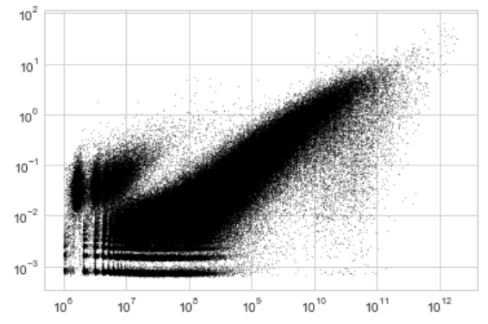
\includegraphics[width=0.8\textwidth]{g2.png}
\end{figure}
\begin{figure}[h]
  \caption{Galaxy formation with log scale (0.5 OR LESS red-shift, Challenging Histogram)}
  \centering
  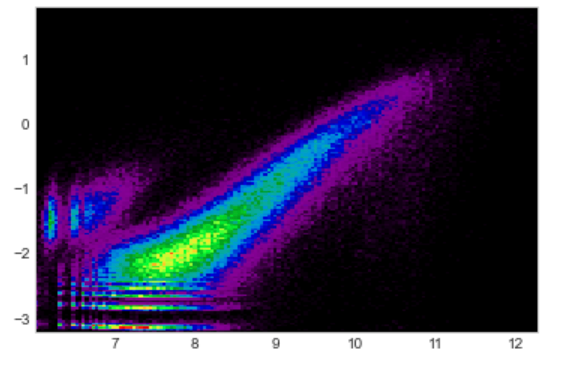
\includegraphics[width=0.8\textwidth]{y.png}
\end{figure}
\newpage

\subsection{Even deeper...}
The image above shows galaxies with red-shift less than 0.5. This corresponds to SnapNum=23 and galaxies as far as back 6 billion years ago. It is more representative and contains many more galaxies than the previous figure as many galaxies are red-shifted because of the expansion of space. Moreover, it has  a higher range of star formation rates with some galaxies going as far as the $10^2$ mark. Notably, the number of galaxies with low masses and high rates of star formation does not change significantly between the red-shifted and non-shifted plots which could imply that many of the young galaxies are close to us. Even though we analyzed galaxies of red shifts 0.5 or lower, we could have chosen red-shifts as large as 20 (SnapNum=0). This is because the universe age is finite (about 13 billion years), so we can't look back more and see higher red-shifts.




\end{document}
